\chapter{解析函数的{\rm Taylor}展开及其应用}
\section{Weierstrass定理}
    对于复数上的数列,其收敛性可以类似于$\mathbb{R}^2$中点集的收敛性即可得到.同样的我们有柯西收敛原理,此处略去\par
    对于复数上的数项级数$\displaystyle{\sum\limits_{n=0}^\infty z_n}$, 
    类似于实数中的常数项级数$\displaystyle{\sum\limits_{n=0}^\infty a_n}$.
    可以定义绝对收敛和条件收敛,以及级数极限的存在性和柯西收敛原理.\par
    下面讨论对于复变函数上的函数项级数$\displaystyle{\sum\limits_{n=1}^\infty f_n(z)}$:

\begin{mypro}
    设$\displaystyle{\sum\limits_{n=1}^\infty f_n(z)}$是定义在$\mathbb{E}$上的级数.
    我们说$\displaystyle{\sum\limits_{n=1}^\infty f_n(z)}$在$\mathbb{E}$上一致收敛到
    $f(z)$.$(\mbox{记为}\ \displaystyle{\sum\limits_{k=1}^n f_k(z)\Rightarrow f(z)})$,
    指$\forall\epsilon>0,\exists.N\in \mathbb{N}^*\quad s.t.\ \forall n>N$.有$\left|S_n(z)-f(z)\right|<\epsilon, \forall z\in E$,
    其中$\displaystyle{S_n(z)=\sum\limits_{k=1}^n f_k(z)}$.
\end{mypro}

\begin{mypro}
    级数$\displaystyle{\sum\limits_{n=1}^\infty f_n(z)}$在$\mathbb{E}$上一致收敛的充要条件是
    $\forall\epsilon>0,\exists.N\in \mathbb{N}^*\quad s.t.\ \forall n>N.\forall p\in N$
    有$\displaystyle{\left|\sum\limits_{i=1}^pf_{n+i}(z)\right|<\epsilon}$.对$\forall z\in\mathbb{E}$均成立.
\end{mypro}
\begin{proof}
    略.
\end{proof}

\begin{mypro}[函数项级数的weierstass判别法,略]
\end{mypro}

\begin{mypro}
    设级数$\displaystyle{\sum\limits_{n=1}^\infty f_n(z)\Rightarrow f(z)}.z\in \mathbb{E},\forall n\in\mathbb{N}^*, f_n\in C(E)$.
    则$f\in C(E)$.
\end{mypro}
\begin{proof}
    $\forall\epsilon>0.\exists N\in\mathbb{N}.\quad s.t.\ n>N$时
    $\displaystyle{\left|f(z)-S_n(z)\right|<\frac{\epsilon}{3}\ \forall z\in\mathbb{E}}$.\\
    对于给定的大于$N$的$n_0$.显然$S_{n_0}\in C(\mathbb{E})$.现任取一个$a\in \mathbb{E}$.故$S_{n_0}$在$a$处连续.\\
    故$\forall\epsilon>0,\exists\delta>0.\quad s.t.\ \forall z\in B(z,\delta)$有
    $\displaystyle{\left|f(z)-f(a)\right|<\frac{\epsilon}{3}}$.\\
    于是$z\in\mathbb{E}\bigcap B(a,\delta)$时有:\\
    $\displaystyle{\left|f(z)-f(a)\right|\leq\left|f(z)-S_{n_0}(z)\right|
    +\left|S_{n_0}(z)-S_{u_0}(a)\right|+\left|S_{u_0}(a)-f(a)\right|<\epsilon}$
\end{proof}

\begin{mypro}
    设级数$\sum\limits_{n=1}^\infty f_u(z)$.在可求长曲线$\gamma$上一致收敛到$f(z)$,若$\forall n\in\mathbb{N}^*,f_n\in C(\gamma),$
    则$\displaystyle{\int_{\gamma}f(z)dz=\sum\limits_{n=1}^\infty\int_{\gamma}f_n(z)dz}$.
\end{mypro}
\begin{proof}
    由定理\emph{4.1.4}.\ $f\in C(\gamma)$.\\
    由于$f_k\Rightarrow f$.故$\forall\epsilon>0.\exists N\in\mathbb{N}^*\quad s.t.\ n>N$时,
    有$\displaystyle{\left|\sum\limits_{k=1}^nf_k(z)-f(z)\right|<\epsilon}.\forall z\in \gamma$.
    故$n>N$时有$\displaystyle{\left|\sum\limits_{k=1}^n\int_\gamma f_k(z)dz-\int_\gamma f(z)dz\right|
    =\left|\int_\gamma\left(\sum\limits_{k=1}^nf_k(z)-f(z)\right)dz\right|<\epsilon\cdot|\gamma|}$
\end{proof}

\begin{mypro}
    若级数$\displaystyle{\sum\limits_{n=1}^\infty f_a(z)}$在区域$\mathbb{D}$的任一紧子集$K$上一致收敛,
    则称$\displaystyle{\sum\limits_{n=1}^\infty f_a(z)}$在$\mathbb{D}$上是内闭一致收敛的.
\end{mypro}
\begin{proof}
    类似于实值函数中的例子,函数项级数$\displaystyle{1+\sum\limits_{k=1}^\infty f_k(z),\ f_k(z)=z^k-z^{k-1}}$
    部分和为$z^k$显然下单位球上内闭一致收敛,但不一致收敛
\end{proof}

\begin{mypro}[Weierstrass I]
    设$D$是$\mathbb{C}$中的域.若$f_n\in C(D),n=1,2\dots\ ,$并且$\displaystyle{\sum\limits_{n=1}^\infty f_n(z)}$在$D$中内闭一致收敛到$f(z)$
    则$f\in H(D)$,并且级数$\displaystyle{\sum\limits_{n=1}^\infty f_n^{(k)}(z)}$在上内闭一致收敛到$f^{(k)}(z).\quad k\in\mathbb{N}$.
\end{mypro}
\begin{proof}
    任取$z_0\in D$,由于$D$为开集,故存在$\delta>0,\quad s.t.\ \overline{B(z_0,\delta)}\subset D$\\
    由定理\emph{4.1.4},$f\in C(\overline{B(z_0,\delta)})$在$B(z_0,\delta)$中任做一个可求长闭曲线$r$,
    由定理\emph{4.1.5}和定理\emph{3.2.4}得$\displaystyle{\int_rf(z)dz=\sum\limits_{n=1}^\infty\int_rf_n(z)dz=0}$.
    故由\emph{Morera}定理得$f\in H(B(z_0,\delta))$\\
    故$f\in H(D)$\\
    任取$\xi\in\partial B(z_0,\delta) ,\forall z\in B(z_0,\frac{\delta}{2})$.
    有$\displaystyle{\left|\frac{1}{(\xi-z)^{k+1}}\right|\leq(\frac{2}{\delta})^{k+1}}$\\
    由一致收敛性得,$\forall\epsilon>0,\ \exists N\in\mathbb{N}^*,\quad s.t.\ \forall n>N,\forall\xi\in\partial B(z_0,\delta)$,有:
    \begin{align*}
        &\left|\sum\limits_{j=1}^nf_j(\xi)-f(\xi)\right|
        <\frac{\epsilon}{k!\cdot\delta}(\frac{\delta}{2})^{k+1}\\
        \Rightarrow&\sum_{j=1}^n\frac{f_j(\xi)}{(\xi-z)^{k+1}}-\frac{f(\xi)}{(\xi-z)^{k+1}}<\frac{\epsilon}{k!\cdot\delta}
    \end{align*}
    故当$z\in B(z_0,\frac{\delta}{2})$时,有:
    \begin{align*}
        \left|\sum\limits_{j=1}^nf_j^{(k)}(z)-f^{(k)}(z)\right|
        &=\frac{k!}{2\pi}\cdot\left|\sum\limits_{j=1}^n\int_{|\xi-z_0|=\delta}\frac{f_j(\xi)d\xi}{(\xi-z)^{k+1}}
        -\int_{|\xi-z_0|=\delta}\frac{f(\xi)d\xi}{(\xi-z)^{k+1}}\right|\\
        &\leq\frac{k!}{2\pi}\int_{|\xi-z_0|=\delta}\left|\sum_{j=1}^n\frac{f_j(\xi)}{(\xi-z)^{k+1}}
        -\frac{f(\xi)}{(\xi-z)^{k+1}}\right|d\xi\\
        &<\epsilon
    \end{align*}
    故$\displaystyle{\sum_{j=1}^nf_j^{(k)}(z)\Rightarrow f^{(k)}(z),z\in B(z_0,\frac{\delta}{2})}$,
    对于$D$的任一紧集$K,K$有有限开球覆盖$SI_kS_{k=1}^n$,故$\displaystyle{\sum\limits_{j=1}^nf_j^{(k)}\Rightarrow f^{(k)}(z),z\in K}$.
\end{proof}

\begin{mypro}[Weierstrass \uppercase\expandafter{\romannumeral2}]
    设$D$为有界区域,对于函数列$\{f_n(z)\}$.有$f_n(z)\in H(D)\bigcap C(\overline{D})$
    且级数$\displaystyle{\sum\limits_{n=1}^\infty f_n(z)}$在$\partial D$上一致收敛,
    则$\displaystyle{\sum\limits_{n=0}^\infty f_n(z)}$在$\overline{D}$上一致收敛.
\end{mypro}
\begin{proof}
    $\forall\epsilon>0,\ \exists N,\ s.t.\ n\geq N, p\geq1$时,有$\left|f_{n+1}(z)+f_{n+2}(z)+\dots+f_{n+p}(z)\right|<\epsilon.$
    对任意$z\in\partial D$均成立,由最大模定理,上述不等式在$\overline{D}$上成立,故级数在$\overline{D}$上一致收敛
\end{proof}

\section{幂函数}
幂级数:$\displaystyle{\sum\limits_{n=0}^\infty} a_n(z-z_0)^n=a_0+a_1(z-z_0)+a_2(z-z_0)^2+\dots+a_n(z-z_0)^n+\dots$\\
其中$a_0,a_1\dots$均为复常数,做平移$\omega=z-z_0$,得$\displaystyle{\sum\limits_{n=0}^\infty z^n=a_0+a_1z+\dots+a_nz^n+\dots(*)}$.
\begin{mypro}
    (收敛半径)(收敛圆).用数分中定义,略
\end{mypro}

\begin{mypro}
    级数$(*)$存在收敛半径$R=(\overline{\lim\limits_{n\to\infty}}\sqrt[n]{|a_n|})^{-1}$,则:\\
    (1)当$R=0$时,$\displaystyle{\sum\limits_{n\equiv0}^\infty a_nz^n}$只在$z=0$处收敛.\\
    (2)当$R=+\infty$时,$\displaystyle{\sum\limits_{n\neq0}^\infty a_nz^n}$在$\mathbb{C}$上收敛.\\
    (3)当$0<R<+\infty$时,$\displaystyle{\sum\limits_{n=0}^\infty a_nz^n}$在$\{z:|z|<R\}$中收敛.在$\{z:|z|>R\}$中发散.
\end{mypro}
\begin{proof}
    同数学分析中的讨论,此处略去
\end{proof}

\begin{mypro}[Abel I]
    如果$\displaystyle{\sum\limits_{n=0}^\infty a_n\cdot z^n}$在$z=z_0\neq0$处收敛,则在$\{z:|z|<z_0\}$中内闭一致收敛.
\end{mypro}
\noindent\emph{证明.}\ 设$K$为$\{z:|z|<|z_0|\}$中的一个紧集,取$r<|z_0|$,使得$k\subset B(0,r)$
\begin{wrapfigure}[4]{r}{2cm}
    \centering
    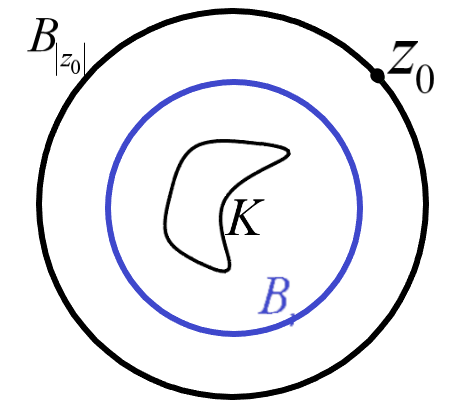
\includegraphics[width=3cm,height=2.7cm]{ch4_p3.png}
\end{wrapfigure}
由于$\displaystyle{\sum\limits_{n=0}^\infty a_nz_0^n}$收敛,故$\left|a_nz_0^n\right|\rightarrow0$
故存在$M\in\mathbb{R}.\ s.t.\ \left|a_nz_0^n\right|<M$\\
故当$z\in k$时,
$\displaystyle{\left|a_k\cdot a^k\right|=\left|a_n\cdot z_o^k\cdot \frac{z^k}{z_0^k}\right|\leq M\left(\left|\frac{z}{z_0}\right|\right)^k}$\\
由于$\displaystyle{\sum\limits_{n=0}^\infty\left|\frac{z}{z_0}\right|^n}$时收敛的,
故由\emph{Weierstrass}判别法得$\displaystyle{\sum\limits_{n=0}^\infty a_nz^n}$在$k$中一致收敛\\\rightline{$\square$}


\noindent 由定理\emph{4.2.3}以及\emph{Weierstrass}定理可以得到:

\begin{mypro}
    幂级数在其收敛圆内确定了一个全纯函数\par
    \qquad\quad\, 那么在收敛圆圆周上的收敛性如何呢?
\end{mypro}

\begin{eg}
    级数$\displaystyle{\sum\limits_{n=0}^\infty z^n}$的收敛半径为1,它在收敛圆周$|z|=1$上处处发散.
\end{eg}

\begin{eg}
    级数$\displaystyle{\sum\limits_{n=0}^\infty \frac{z^n}{n^2}}$的收敛半径为1,它在收敛圆周$|z|=1$上处处收敛.
\end{eg}

\begin{eg}
    级数$\displaystyle{\sum\limits_{n=0}^\infty \frac{z^n}{n}}$的收敛半径为1,
    它在收敛圆周$|z|=1$上在$z=e^{i\theta}(0<\theta<2\pi)$处收敛,在1处发散.
\end{eg}

\begin{proof}
    显然$z=1$时级数时发散的\\
    当$\theta\neq0$时$\displaystyle{\sum\limits_{n=0}^\infty\frac{z^n}{n}=
    \sum\limits_{n=0}^\infty\frac{\cos n\theta}{n}+i\cdot\sum\limits_{n=0}^\infty \frac{\sin n\theta}{n}}$
    由实数项级数的\emph{Dirichlet}判别法,\\
    得$\displaystyle{\sum\limits_{n=0}^\infty\frac{\cos n\theta}{n},\ \sum\limits_{n=0}^\infty \frac{\sin n\theta}{n}}$收敛\\
\end{proof}
由上述例子可知,收敛圆周上的收敛性无法确定\par 这也是我们下面要探讨的问题\par
设级数$\displaystyle{\sum\limits_{n=0}^\infty a_n(z-z_0)^n}$的收敛半径为$R$,
我们来研究$\displaystyle{\xi\in B(z_0,R),\sum\limits_{n=0}^\infty a_n(\xi-z_0)^n}$与和函数$f$的关系:
令$\displaystyle{\omega=\frac{z-z_0}{\xi-z_0}}$
故$\omega\in B(0,1)$,级数可改写为$\displaystyle{\sum\limits_{n=0}^\infty b_n\omega^n},b_n=a_n(\xi-z_0)^n$,
故新的幂级数的收敛半径为1,故以下我们在收敛半径为1的情况下做讨论.

\begin{mypro}[*]
    设$g$是定义在单位圆中的函数,$e^{i\theta_0}$是单位圆上的一点,记$S_\alpha(e^{i\theta_0})$为以$e^{i\theta_0}$为顶点,
    以$e^{i\theta_0}$点对应的极径在单位圆内侧向两侧张出的张角为$2\alpha$
    的角形区域$(\alpha<\frac{\pi}{2})$
\end{mypro}

\begin{wrapfigure}[2]{r}{3cm}
    \centering
    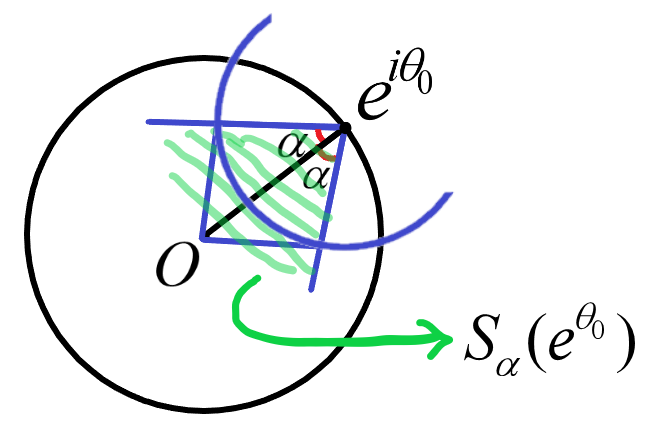
\includegraphics[width=3cm,height=2cm]{ch4_p4_1st.png}
\end{wrapfigure}
\noindent \emph{若$z$在$S_\alpha(e^{i\theta_0})$中趋于$e^{i\theta_0}$时$g(z)$有极限$C$则称$g$在$\theta_0$处有非切向极限$C$,记为
$\displaystyle{\lim\limits_{\substack{z\to e^{i\theta_0}\\z\in S_\alpha(e^{i\theta_0})}}g(z)=C}$}
\\
\\
\begin{mypro}[*](\rm Abel \uppercase\expandafter{\romannumeral2})
    设$\displaystyle{f(z)=\sum\limits_{n=0}^\infty a_nz^n}$的收敛半径为$R=1$,
    且级数在$z=1$处收敛于$S$,则$f$在$z=1$处有非切向极限$S$
\end{mypro}
\noindent\emph{证明.}
记$\displaystyle{\sigma_{n,\rho}=\sum\limits_{i=1}^p a_{n+i}}$由条件得$\displaystyle{\sum\limits_{n=0}^\infty a_n}$收敛.\\
故$\forall\epsilon>0 ,\ \exists$正整数$N,\  s.t.\ $当$n>N$时,对任意自然数$p$有$|\sigma_{n,p}|<\epsilon$\\
由于
\begin{align*}
    \sum\limits_{i=1}^pa_{n+i}\cdot z^{n+i}&=\sum\limits_{i=1}^{p-1}(\sigma_{n,i+1}-\sigma_{n,i})z^{n+1+i}+\sigma_{n,1}z^{n+1}\\
    &=\sum\limits_{i+1}^{p-1}\sigma_{n,i}z^{n+i}\cdot(1-z)+\sigma_{n,p}z^{n+p}\\
    &=z^{n+1}(1-z)\cdot\sum\limits_{i=1}^{p-1}(\sigma_{n,i}\cdot z^{i-1})+\sigma_{n,p}\cdot z^{n+p}
\end{align*}
故当$|z|<1,n>N$.时有:$\displaystyle{\left|\sum\limits_{i=1}^pa_{n+i}\cdot z^{n+i}\right|
<\epsilon\cdot|1-z|\cdot\sum\limits_{n=p}^\infty|z^n|+\epsilon=\epsilon\left(\frac{|1-z|}{1-|z|}+1\right)}$\\
任取$\displaystyle{z\in S_\alpha(1)\cap B(1,\delta)}$记$|z|=r,|1-z|=\rho$则由余弦定理得$r^2=1+\rho-2\rho\cos\theta$\\
\begin{wrapfigure}[3]{r}{3cm}
    \centering
    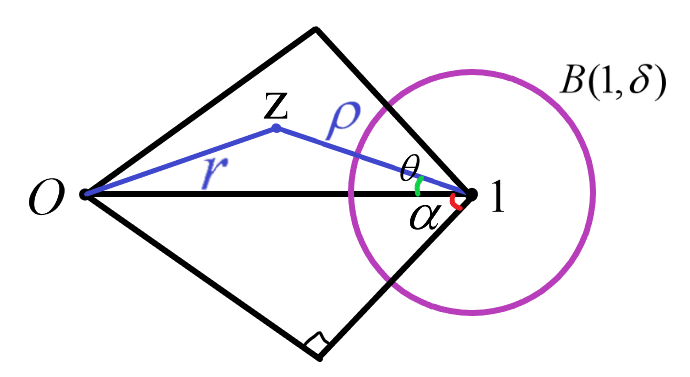
\includegraphics[width=3.5cm,height=2.0cm]{ch4_p4_2nd.png}
\end{wrapfigure}
故$\displaystyle{\frac{|1-z|}{1-|z|}=\frac{\rho}{1-r}=\frac{\rho(1+r)}{1-r^2}
\leq\frac{2\rho}{2\rho\cos\theta-\rho^2}=\frac{2}{2\cos\theta-\rho}}$\\
又由于$z\in B(1,\delta).$故$\rho<\delta<\cos\alpha<\cos\theta$故$\displaystyle{\frac{|1-z|}{1-|z|}<\frac{2}{\cos\alpha}}$\\
故$\displaystyle{\left|\sum\limits_{i=1}^pa_{n+i}\cdot z^{n+i}\right|<\epsilon(\frac{2}{\cos\alpha}+1)}$
,故$\displaystyle{\sum\limits_{n=0}^\infty a_nz^n}$在$\displaystyle{S_\alpha(1)\cap B(1,\delta)}$上一致收敛
设和函数为$f$,由一致收敛性得$f$在$\displaystyle{S_\alpha(1)\cap B(1,\delta)}$上连续,
故$\displaystyle{\lim\limits_{\substack{z\in S_\alpha(1)\\z\to 1}}f(z)=f(1)=S}$\\\rightline{$\square$}
